% Options for packages loaded elsewhere
% Options for packages loaded elsewhere
\PassOptionsToPackage{unicode}{hyperref}
\PassOptionsToPackage{hyphens}{url}
\PassOptionsToPackage{dvipsnames,svgnames,x11names}{xcolor}
%
\documentclass[
  portuguese,
]{estat/estat}
\usepackage{xcolor}
\usepackage[left=3cm,right=2cm,top=3cm,bottom=2cm]{geometry}
\usepackage{amsmath,amssymb}
\setcounter{secnumdepth}{5}
\usepackage{iftex}
\ifPDFTeX
  \usepackage[T1]{fontenc}
  \usepackage[utf8]{inputenc}
  \usepackage{textcomp} % provide euro and other symbols
\else % if luatex or xetex
  \usepackage{unicode-math} % this also loads fontspec
  \defaultfontfeatures{Scale=MatchLowercase}
  \defaultfontfeatures[\rmfamily]{Ligatures=TeX,Scale=1}
\fi
\usepackage{lmodern}
\ifPDFTeX\else
  % xetex/luatex font selection
  \setmainfont[]{Arial}
\fi
% Use upquote if available, for straight quotes in verbatim environments
\IfFileExists{upquote.sty}{\usepackage{upquote}}{}
\IfFileExists{microtype.sty}{% use microtype if available
  \usepackage[]{microtype}
  \UseMicrotypeSet[protrusion]{basicmath} % disable protrusion for tt fonts
}{}
\makeatletter
\@ifundefined{KOMAClassName}{% if non-KOMA class
  \IfFileExists{parskip.sty}{%
    \usepackage{parskip}
  }{% else
    \setlength{\parindent}{0pt}
    \setlength{\parskip}{6pt plus 2pt minus 1pt}}
}{% if KOMA class
  \KOMAoptions{parskip=half}}
\makeatother
% Make \paragraph and \subparagraph free-standing
\makeatletter
\ifx\paragraph\undefined\else
  \let\oldparagraph\paragraph
  \renewcommand{\paragraph}{
    \@ifstar
      \xxxParagraphStar
      \xxxParagraphNoStar
  }
  \newcommand{\xxxParagraphStar}[1]{\oldparagraph*{#1}\mbox{}}
  \newcommand{\xxxParagraphNoStar}[1]{\oldparagraph{#1}\mbox{}}
\fi
\ifx\subparagraph\undefined\else
  \let\oldsubparagraph\subparagraph
  \renewcommand{\subparagraph}{
    \@ifstar
      \xxxSubParagraphStar
      \xxxSubParagraphNoStar
  }
  \newcommand{\xxxSubParagraphStar}[1]{\oldsubparagraph*{#1}\mbox{}}
  \newcommand{\xxxSubParagraphNoStar}[1]{\oldsubparagraph{#1}\mbox{}}
\fi
\makeatother


\usepackage{longtable,booktabs,array}
\usepackage{calc} % for calculating minipage widths
% Correct order of tables after \paragraph or \subparagraph
\usepackage{etoolbox}
\makeatletter
\patchcmd\longtable{\par}{\if@noskipsec\mbox{}\fi\par}{}{}
\makeatother
% Allow footnotes in longtable head/foot
\IfFileExists{footnotehyper.sty}{\usepackage{footnotehyper}}{\usepackage{footnote}}
\makesavenoteenv{longtable}
\usepackage{graphicx}
\makeatletter
\newsavebox\pandoc@box
\newcommand*\pandocbounded[1]{% scales image to fit in text height/width
  \sbox\pandoc@box{#1}%
  \Gscale@div\@tempa{\textheight}{\dimexpr\ht\pandoc@box+\dp\pandoc@box\relax}%
  \Gscale@div\@tempb{\linewidth}{\wd\pandoc@box}%
  \ifdim\@tempb\p@<\@tempa\p@\let\@tempa\@tempb\fi% select the smaller of both
  \ifdim\@tempa\p@<\p@\scalebox{\@tempa}{\usebox\pandoc@box}%
  \else\usebox{\pandoc@box}%
  \fi%
}
% Set default figure placement to htbp
\def\fps@figure{htbp}
\makeatother



\ifLuaTeX
\usepackage[bidi=basic]{babel}
\else
\usepackage[bidi=default]{babel}
\fi
\ifPDFTeX
\else
\babelfont{rm}[]{Arial}
\fi
% get rid of language-specific shorthands (see #6817):
\let\LanguageShortHands\languageshorthands
\def\languageshorthands#1{}


\setlength{\emergencystretch}{3em} % prevent overfull lines

\providecommand{\tightlist}{%
  \setlength{\itemsep}{0pt}\setlength{\parskip}{0pt}}



 


\authors{%
    Estatiano 1 \\
    Estatiano 2\\
    Estatiano 3\\
}

% escreva o nome do cliente aqui
% se for mais de um separe por \\
\client{%
    ESTAT
}
% Baixando pacotes
\RequirePackage{fancyhdr}
\RequirePackage{graphicx}

\setlength\headheight{28pt}  

\setlength{\parindent}{15pt} % Adiciona indentação nos parágrafos
\setlength{\parskip}{0pt} % Adiciona 0 espaço entro os parágrafos

\let\oldsection\section
\renewcommand\section{\clearpage\oldsection}
\makeatletter
\@ifpackageloaded{float}{}{\usepackage{float}}
\floatstyle{plain}
\@ifundefined{c@chapter}{\newfloat{quadro}{h}{loquad}}{\newfloat{quadro}{h}{loquad}[chapter]}
\floatname{quadro}{Quadro}
\floatstyle{plaintop}
\restylefloat{quadro}
\newcommand*\listofquadros{\listof{quadro}{List of Testes}}
\makeatother
\makeatletter
\@ifpackageloaded{caption}{}{\usepackage{caption}}
\AtBeginDocument{%
\ifdefined\contentsname
  \renewcommand*\contentsname{Índice}
\else
  \newcommand\contentsname{Índice}
\fi
\ifdefined\listfigurename
  \renewcommand*\listfigurename{Lista de Figuras}
\else
  \newcommand\listfigurename{Lista de Figuras}
\fi
\ifdefined\listtablename
  \renewcommand*\listtablename{Lista de Tabelas}
\else
  \newcommand\listtablename{Lista de Tabelas}
\fi
\ifdefined\figurename
  \renewcommand*\figurename{Figura}
\else
  \newcommand\figurename{Figura}
\fi
\ifdefined\tablename
  \renewcommand*\tablename{Tabela}
\else
  \newcommand\tablename{Tabela}
\fi
}
\@ifpackageloaded{float}{}{\usepackage{float}}
\floatstyle{ruled}
\@ifundefined{c@chapter}{\newfloat{codelisting}{h}{lop}}{\newfloat{codelisting}{h}{lop}[chapter]}
\floatname{codelisting}{Listagem}
\newcommand*\listoflistings{\listof{codelisting}{Lista de Listagens}}
\captionsetup{labelsep=colon}
\makeatother
\makeatletter
\makeatother
\makeatletter
\@ifpackageloaded{caption}{}{\usepackage{caption}}
\@ifpackageloaded{subcaption}{}{\usepackage{subcaption}}
\makeatother
\usepackage{bookmark}
\IfFileExists{xurl.sty}{\usepackage{xurl}}{} % add URL line breaks if available
\urlstyle{same}
\hypersetup{
  pdflang={pt},
  colorlinks=true,
  linkcolor={black},
  filecolor={black},
  citecolor={black},
  urlcolor={black},
  pdfcreator={LaTeX via pandoc}}


\author{}
\date{}
\begin{document}

% Limpando tudo
\fancyhf{} 

% Ajustes do header
\fancyhead[L]{} % limpando o lado esquerdo
\fancyhead[R]{
\includegraphics[width=0.20\textwidth]{estat/imagens/estat.png}} % adicionando logo no canto direito
\renewcommand{\headrulewidth}{0pt}   % sem linha embaixo da logo

% Ajustes de fim de página
\fancyfoot[R]{\textcolor{white}{\thepage}} % Número em branco no canto direito

% Aplicando o estilo que acabamos de criar
\pagestyle{fancy} 


\labelformat{quadro}{\textbf{#1}}

\renewcommand*\contentsname{Sumário}
{
\hypersetup{linkcolor=}
\setcounter{tocdepth}{3}
\tableofcontents
}

\section{Análises}\label{anuxe1lises}

\subsection{Análise das receitass médias das loja registradas nos anos
de 1880 até
1889}\label{anuxe1lise-das-receitass-muxe9dias-das-loja-registradas-nos-anos-de-1880-atuxe9-1889}

Esta análise, busca-se compreender a tendência da receita média anual no
período de 10 anos, entre 1880 até 1889, com o objetivo de entender se
teve um aumento ou diminuição no faturamento realizado em cada ano. Na
análise será utilizado a variável receita média, que é quantitativa
contínua e ano de vendas, uma variável quantitativa discreta. Será
utilizado a cotação atual do dólar, em R\$ 5,31. A amostra traz a média
do volume de vendas de 18 lojas registradas nesse período. A
visualização e entendimento da evolução da receita média em cada ano
será através de um gráfico de linhas, sendo o mais adequado para essa
análise e de uma tabela, onde os principais dados utilizados estarão
reunidos.

\begin{figure}[H]

\caption{\label{fig-receita_media}Gráfico de linhas da receita média
anual de 1880 a 1889}

\centering{

\pandocbounded{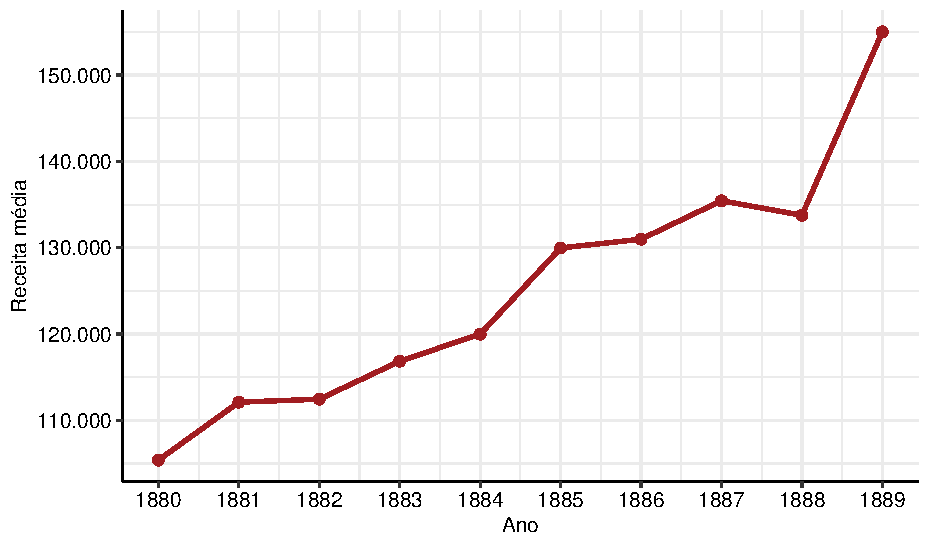
\includegraphics[keepaspectratio]{entrega_1_files/figure-pdf/fig-receita_media-1.pdf}}

}

\end{figure}%

\begin{table}[H]

\caption{\label{tbl-receita_media}}

\centering{

\begin{tabular}{c|c|c}
\toprule
\textbf{Anos} & \textbf{Média das receitas} & \textbf{Porcentagem de aumento} \\
\midrule
1880 & 105.399,0 & - \\
1881 & 112.110,0 & 6,37\% \\
1882 & 112.452,4 & 0,31\% \\
1883 & 116.856,9 & 3,92\% \\
1884 & 119.989,8 & 2,68\% \\
1885 & 129.969,0 & 8,32\% \\
1886 & 130.989,2 & 0,78\% \\
1887 & 135.444,8 & 3,40\% \\
1888 & 133.757,6 & −1,25\% \\
1889 & 155.009,1 & 15,89\% \\
\midrule
\textbf{Total} & 1.252.977,8 & 47,07\% \\
\bottomrule
\end{tabular}

}

\end{table}%

Através do gráfico \(\ref{fig-receita_media}\) e da tabela
\ref{tbl-receita_media} é possível entender o aumento das receitas
médias ao longo dos anos. Em 1883, houve um acréscimo de 10,83\% na
receita média em relação a 1880. Esses dados indicam que existe uma
tendência de aumento na receita média ao longo desses anos. Em 1886,
teve um acréscimo de 24,28\% em comparação com 1880, tendo um aumento de
12,09\% em relação a 1883. Isso reforça a tendência de crescimento
observada ao longo dos anos. Em 1887 teve um queda de 1,25\%, sendo o
úncio ano onde teve uma diminuição na receita, mostrando que esse ano
foi atípico. Em contra partida em 1889, teve um aumento de 47,07\% em
relação a 1880, sendo o maior salto de receita entre 1888 e 1889, onde
foi de 15,89\%. Observa-se que nessa década teve uma aceleração no
crescimento das receitas médias ao longo dos anos, com o maior impulso
de crescimento registrado no ano final.




\end{document}
